\documentclass[a4paper,10pt,usenames]{article}
%\documentclass[color=pdftex]{beamer}
\usepackage[T2A]{fontenc}
\usepackage[utf8x]{inputenc}
\usepackage{ucs}
\usepackage{cmap}
\usepackage[english,russian]{babel}
\usepackage{amsmath}
\usepackage{graphicx}
\usepackage{indentfirst}
\usepackage{ucs} 
\usepackage[utf8x]{inputenc}
\usepackage{caption}
\usepackage{placeins}
\usepackage{listings}
\usepackage{hyperref}
\usepackage{amsfonts}
\usepackage[usenames,dvipsnames]{color}    
\lstset{ 
  language=R,                     % the language of the code
  basicstyle=\small\ttfamily, % the size of the fonts that are used for the code
  numbers=left,                   % where to put the line-numbers
  numberstyle=\small\color{Blue},  % the style that is used for the line-numbers
  stepnumber=1,                   % the step between two line-numbers. If it's 1, each line
                                  % will be numbered
  numbersep=5pt,                  % how far the line-numbers are from the code
  backgroundcolor=\color{white},  % choose the background color. You must add \usepackage{color}
  showspaces=false,               % show spaces adding particular underscores
  showstringspaces=false,         % underline spaces within strings
  showtabs=false,                 % show tabs within strings adding particular underscores
  frame=single,                   % adds a frame around the code
  rulecolor=\color{black},        % if not set, the frame-color may be changed on line-breaks within not-black text (e.g. commens (green here))
  tabsize=2,                      % sets default tabsize to 2 spaces
  captionpos=b,                   % sets the caption-position to bottom
  breaklines=true,                % sets automatic line breaking
  breakatwhitespace=false,        % sets if automatic breaks should only happen at whitespace
  keywordstyle=\color{RoyalBlue},      % keyword style
  commentstyle=\color{YellowGreen},   % comment style
  stringstyle=\color{ForestGreen}      % string literal style
} 


\title{Исследование спайкового кода}
\author{Чернышев Алексей}
\setlength{\parindent}{1cm}
\def\la{\left\langle\rule{0pt}{3em}}
\def\ra{\right\rangle}
\newcommand{\HRule}{\rule{\linewidth}{0.5mm}}



\begin{document}

{ \huge \bfseries Исследование спайкового кода \\[0.4cm] }


\tableofcontents
\clearpage
\section{Спайковый код}
\indent Спайк - элементарная единица информации, которой обмениваются биологические нейроны. Соединённые синаптическими связями, нейроны, сложно и нелинейно перерабатывая вход с синапсов, вырабатывают на своём выходе (аксон нейрона), короткие электрохимические импульсы. В анализе удобно рассматривать спайки, как бинарные события (рис. \ref{spiking_neuron_pic}). 
\begin{figure}[ht]
\centering
\captionsetup{justification=centering,margin=1cm}
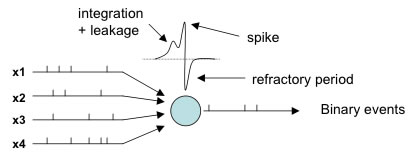
\includegraphics[width=75mm,scale=0.7]{spiking_neuron.jpg}
\caption{Спайковый нейрон}
\label{spiking_neuron_pic}
\end{figure}\\
\indent То как нейроны кодируют информацию в спайках, очень живой и трепещущий вопрос для современного научного сообщества. Важный нюанс спайкового кода в том, что он не надёжен. Исследования показали, что на один и тот же стимул популяция нейронов может дать разный ответ, что даёт огромное пространство для интерпретаций. \\
\indent На протяжении 20-ого века большинство нейрофизиологов было убеждено, что ненадёжность разрешается, если усреднять спайки на некотором промежутке времени (около 100 мс), и вся информация хранится в средних активностях нейронов. Однако, в конце 20-ого века было проведено множество исследований, показавших, что достаточно много информации хранится в самих временах спайков, и что усреднение, только ухудшает декодирование информации полученной от нейронов.\\
\indent В данном задании будет возможность закодировать сигнал в виде спайкового кода, через симуляцию популяции нейронов. Получив ответ в виде спайков, мы его декодируем, и необходимо будет сделать анализ полученных результатов, при помощи инструментов данных в этом руководстве.\\
\section{Спайковый нейрон}
\indent На рис. \ref{spiking_neuron_pic}, также, показан типичный профиль активности нейрона, основные свойство которого: 
\begin{itemize}
\item интеграция входного сигнала (integration);
\item угасание этого сигнала на нейроне со временем, или иначе говоря ``утечка'' (leakage);
\item рефракторный период, нейрон переживает его после выработки спайка, как следствие сложных химических реакций, некоторое время (от 2-10 мс) неработоспособен.
\end{itemize}
\indent Моделирование спайковых нейронов в виде наиболее приближенном к биологии, насколько позволяет современная нейронаука, возможно, но очень трудозатратно с точки зрения ресурсов компьютера. Существует модели, более менее, приближенные к биологическому аналогу и которые не так сложно моделировать. Две из них будут рассмотрены в задании.
\subsection{Модель Integrate-and-fire}
\indent Самая простая спайковая модель, основанная на RC цепи, записывается в виде дифференциального уравнения
   \begin{equation}\label{eq:iaf}
   \tau_{m}\frac{du}{dt} =-u+R I(t),
   \end{equation}
при $u \geq \vartheta$ потенциал мембраны сбрасывается и на $\tau_{ref}$ держится в сброшенном состоянии
   \begin{equation}\label{eq:iaf_reset}
   u \leftarrow u_{r} \mbox{ в течении }\tau_{ref}, 
   \end{equation}
   где $\vartheta$ - порог напряжения, временная константа мембраны $\tau_{m}=RC$, $R$ и $C$ - сопротивление и ёмкость RC-цепи соответственно, $\tau_{ref}$ - рефракторное время, $I(t)$ - приложенный ток извне, $u_{r}$ - константа описывающая потенциал мембраны покоя нейрона.\\
   \indent Пример работы такого нейрона можно посмотреть на рис.\ref{iaf_neuron_pic}.\\
\begin{figure}[ht]
\centering
\captionsetup{justification=centering,margin=1cm}
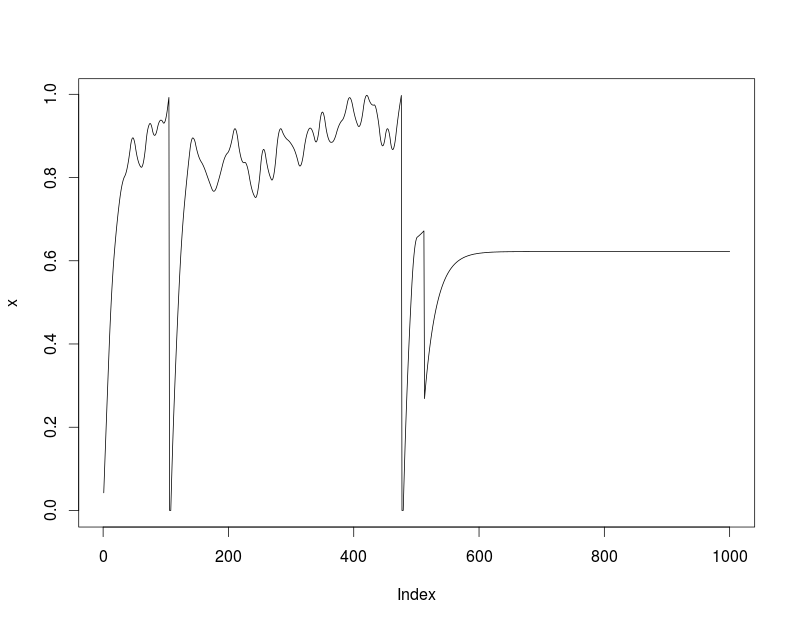
\includegraphics[width=120mm,scale=1]{iaf_profile.png}
\caption{Напряжение на мембране IaF, при $u_{r} = 0, \vartheta = 1, \tau_{ref} = 2$ мс, $\tau_{m} = 20$ мс}
\label{iaf_neuron_pic}
\end{figure}\\
\subsection{Модель Adaptive Exponential Integrate-and-fire}
\indent Более сложная, но более приближенная к биологии модель спайкового нейрона, описывается системой дифференциальных уравнений с двумя переменными. Основная особенность поведения системы, в том, что нейрон адаптируется, т.е. со временем показывает меньшую активность при одинаковой характеристике входа

\begin{align}
C\frac{du}{dt} &= -g_{L}(V-E_{L}) + g_{L}\Delta_{T}exp\left(\frac{V-V_{T}}{\Delta_{T}}\right)-w+I(t) \nonumber\\
\tau_{w}\frac{dw}{dt}&=a(V-E_{L})-w
\end{align}
Генерация спайка происходит аналогично обычной модели IaF:
   \begin{equation}\label{eq:iaf_reset}
   u \leftarrow u_{r} \mbox{ в течении }\tau_{ref}, 
   \end{equation}
\begin{figure}[ht]
\centering
\captionsetup{justification=centering,margin=1cm}
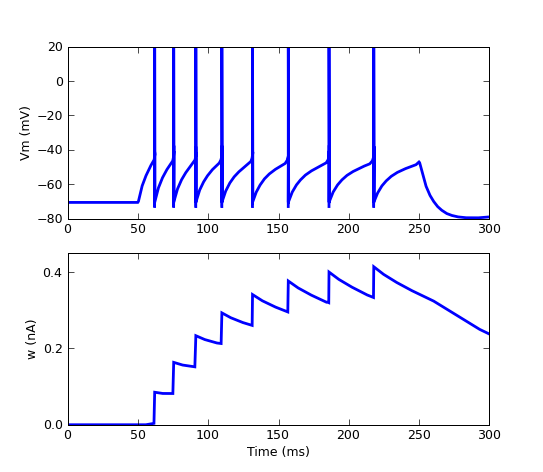
\includegraphics[width=120mm,scale=1]{AdExRS.png}
\caption{Поведение переменных AdEx IaF}
\label{adex_iaf_neuron_pic}
\end{figure}\\
\subsection{Кодирование спайковым кодом}
\indent Задача кодирования спайковым кодом временного ряда $X(t)$ популяцией $N$ нейронов, заключается в том, чтобы найти такое преобразование $X(t)\rightarrow I_{i}(t)$, для, $i\in\{1,..,N\}$, которое является наиболее оптимальным по данному критерию оценки.\\
\indent В качестве критерия оценки возьмём качество линейного восстановления сигнала $X(t)$ из спайкового кода.	

\subsubsection{Линейная кривая настройки}
\indent Под линейной кривой настройки понимается, что нейрон чувствителен к определённому значению временного ряда, причём частота его спайков, линейно возрастает с возрастанием или убыванием значения
\begin{figure}[ht]
\centering
\captionsetup{justification=centering,margin=1cm}
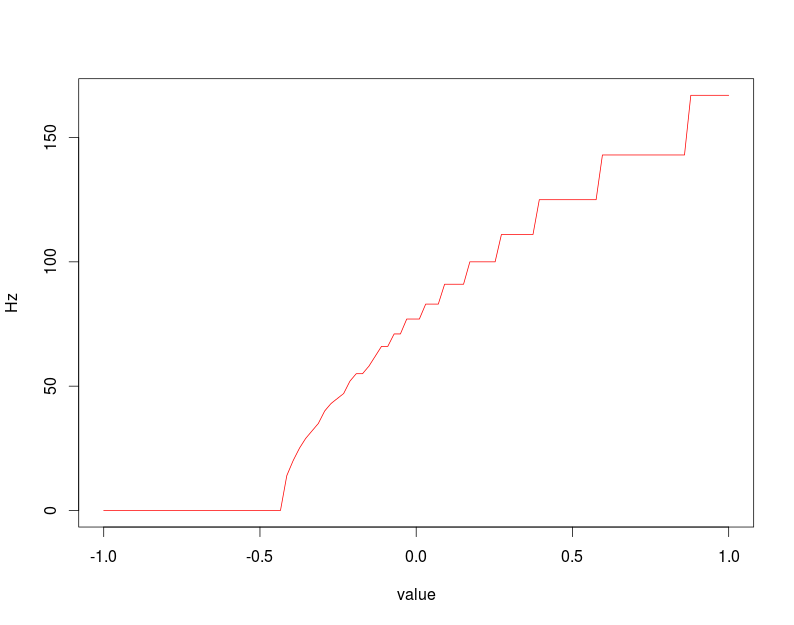
\includegraphics[width=120mm,scale=1]{linear_curve.png}
\caption{Линейная кривая настройки}
\label{linear_curve}
\end{figure}\\
Как для IaF, так и для AdEx IaF, такая кривая настройки задаётся преобразованием
\begin{equation}
I_{i}(t) = g_{i}X(t) + b_{i}
\end{equation} 
где $g_{i}, b_{i} \in \mathbb{R}$ -- усиление и смещение преобразования, соответственно.\\
\subsubsection{Сигмоидная кривая настройки}
\indent Сигмодная кривая настройки получается преобразованием вида
\begin{equation}
I_{i}(t) = g^{s}_{i}exp\left(-\frac{(X(t)-C_{i})^2}{2\sigma_{i}^2} \right)
\end{equation}
где $g^{s}_{i}, C_{i}, \sigma_{i} \in \mathbb{R}$ -- усиление, центр и разброс сигмоидной кривой, соответственно.\\
На рисунке показан типичной профиль этой кривой настройки
\begin{figure}[ht]
\centering
\captionsetup{justification=centering,margin=1cm}
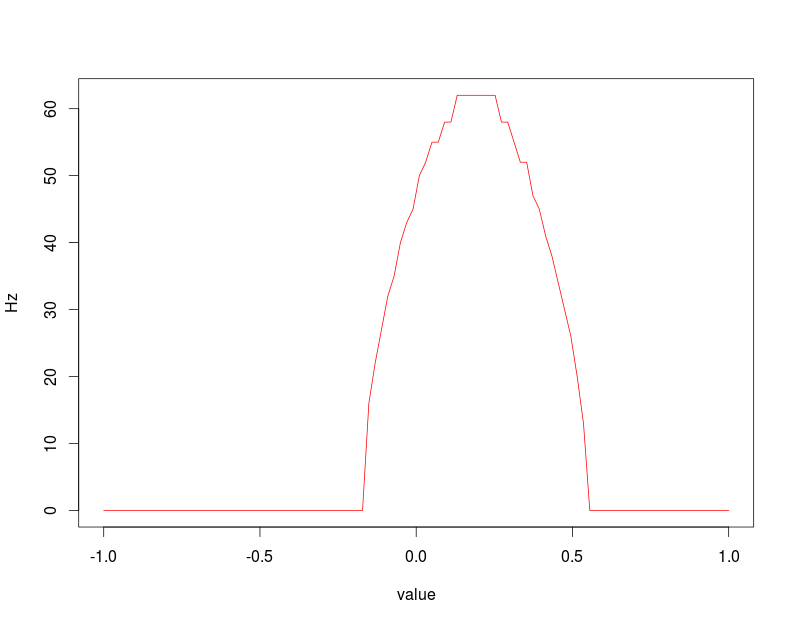
\includegraphics[width=120mm,scale=1]{sigma_curve.png}
\caption{Сигмоидная кривая настройки}
\label{sigma_curve}
\end{figure}\\
\subsubsection{Критерий оценки}
\indent В качестве критерия оценки возьмём качество линейного восстановления исходного сигнала $X(t)$. Фильтр Винера -- один из самых известных и простых линейных фильтров. После обучения фильтра, фильтр с тем или иным качеством восстанавливает сигнал, и это качество можно выразить отношением сигнал-шум:
\begin{equation}
SNR=\frac{X(w)}{X(w)-X'(w)},
\end{equation}
где $X'(w),X(w)$ -- восстановленный сигнал и исходный сигнал в частотном домене.\\
\indent В качестве базовой метрики качества спайкового кодирования возьмум информацию на каждый частотный канал:
\begin{equation}\label{eval}
Info = \frac{1}{2}log_{2}(1+SNR)
\end{equation}
\subsection{Задание}
\indent Основная задача состоит в исследовании влияения параметров кривых настроек и нейрона на критерий оценки \eqref{eval}. Провести мета-оптимизацию по параметрам для максимизации критерия.\\
\textbf{Вариант 1.} Исследование линейных кривых настроек для определенных данных. Мета-оптимизация методом \textit{cma-es}.\\
\textbf{Вариант 2.} Исследование сигмоидных кривых настроек и настроек нейрона для определенных данных. Мета-оптимизация методом \textit{GP}. \\
\subsection{Материалы}
Нейронные модели, кривые настройки, оптимизация фильтров Винера находятся в репозитории:\\
\url{https://github.com/alexeyche/snn_sim.git} \\ 
\indent Репозиторий содержит научный проект в виде библиотеки на C, который имеет, как обычную точку входа в виде программ, так и пакет для языка \textbf{R}.\\
\indent Для того чтобы собрать пакет для \textbf{R}, необходимо собрать и установить библиотеку:
\begin{lstlisting}
$ git clone https://github.com/alexeyche/snn_sim.git
$ mkdir snn_sim/build
$ cd snn_sim/build 
$ cmake ../sources
$ make -j8
$ sudo make install
\end{lstlisting}
далее, для сборки пакета \textbf{R} необходимо выполнить скрипт:
\begin{lstlisting}
$ cd ../r_package
$ ./build.sh 
\end{lstlisting}
Примеры построения кривых настроек можно посмотреть в скриптах, для линейных кривых:\\
\begin{lstlisting}
snn_sim/r_package/r_scripts/linear_curves_test.R
\end{lstlisting}
для сигмоидных кривых: \\
\begin{lstlisting}
snn_sim/r_package/r_scripts/sigma_curves_test.R
\end{lstlisting}
\end{document}
